\documentclass[14pt, table]{beamer}
%\documentclass[14pt, table, handout]{beamer}
%\usetheme{Luebeck}
\usetheme{Malmoe}
%\usetheme{Pittsburgh}
%\usetheme{Rochester}
%\usetheme{metropolis}

\usecolortheme{spruce}
%\usecolortheme{beaver}

% Get rid of footer
\setbeamertemplate{navigation symbols}{}
\setbeamertemplate{footline}{}

% Speaker notes
%\setbeameroption{show only notes}
%\setbeameroption{show notes}
%\setbeameroption{show notes on second screen}
\setbeamerfont{note page}{size=\footnotesize}
\addtobeamertemplate{note page}{
	\setbeamerfont{itemize/enumerate subbody}{size=\footnotesize}}{}
	
% highlighting
\usepackage{graphicx}
\usepackage{soul}

% Graphics and such
\usepackage{booktabs}
\usepackage[RPvoltages]{circuitikz}
\ctikzset{logic ports=ieee,logic ports/scale=1}

\usetikzlibrary{decorations.pathmorphing}
\usetikzlibrary{calc, positioning}
\usetikzlibrary{shapes.arrows, fadings}

\newcommand{\bigkey}[1] {
	\draw (#1) ++ (20:.5) coordinate (top) arc(20:340:.5) coordinate (bottom);
	\draw (#1) ++ (-.2,0) circle (.1);
	\draw (#1) ++ (.5,.1) -- ++ (1,0);
	\draw (top) -- ++(1.25,0)
	coordinate (tmp) -- ($(#1 -| tmp) + (.15,0)$)
	coordinate (tip);
	\draw [decorate, decoration={
		zigzag,
		segment length=10,
		amplitude=2.5,
		pre length = 5.57, % centers zigzag
		post length = 0
	}] (bottom) -- ++(1.25,0) coordinate (tmp);
	\draw (tmp) -- (tip);
}

\newcommand{\littlekey}[2] {
	\draw (#1)++(-.4,0) coordinate (center);
	\draw (center) node[] {\tiny{#2}};
	\draw (center)++ (20:.3) coordinate (top) arc(20:340:.3) coordinate (bottom);
	\draw (center)++ (-.2,0) circle (.05);
	%\draw (center)++ (.5,.1) -- ++ (.75,0);
	\draw (top) -- ++(.7,0)
	coordinate (tmp) -- ($(#1 -| tmp) + (.15,0)$)
	coordinate (tip);
	\draw [decorate, decoration={
		zigzag,
		segment length=5,
		amplitude=1,
		pre length = 2.5, % centers zigzag
		post length = 0
	}] (bottom) -- ++(.7,0) coordinate (tmp);
	\draw (tmp) -- (tip);
}

\newcommand{\lockshape}[2]{
	\draw (#1) ++ (-.7,.7) node [below right] {\footnotesize{#2}};
	\draw[thick] (#1) ++ (-60:.1) coordinate (right)
	arc (-60:240:.1)
	-- ++ (0,-.2) -| (right);
	\node[rectangle, draw, thick, minimum size=30] at (#1) (lastBox) {};
	%\draw (#1) ++ (-.7,.7) rectangle ++(1.4,-1.4);
}

\newcommand{\examplecircuit}[5] {
	\begin{tikzpicture}
		\node[xor port] (xor)  at (0, 0){};
		\node[and port] (andA) at (3, .7){};
		\node[and port] (andB) at (3,-.7){};
		\draw (andA.in 1)  -- ++(-5, 0)
		      (andB.in 2)  -- ++(-5, 0)
		      (xor.in 1)   -| ++(-1, .7) node [below right] {#1}
		      (xor.in 2)   -| ++(-1,-.7) node [above right] {#2}
		      (andA.in 2)  -| (xor.out)  node [      right] {#3}
		      (andB.in 1)  -| (xor.out)
		      (andA.out) node [above] {#4} -- ++( 1, 0)
		      (andB.out) node [above] {#5} -- ++( 1, 0)
		      (0,-2); % force a bit of padding
	\end{tikzpicture}
}


\title{Multi-Party Computation}
\subtitle{Yao's Garbled Circuits}
\author{Gabriel Kulp}
\institute{kulpga@oregonstate.edu}

\begin{document}
\maketitle{}
\note{
My name is Gabriel Kulp and I'm going to present an introduction to Multi-Party Computation, a field of cryptography that you might not have heard of. Specifically, I will describe Yao's Garbled Circuits protocol.

}

\begin{frame}{What is Multi-Party Computation?}
	\begin{itemize}[<+->]
		\item MPC = multi-party computation
		\item Interactive cryptographic protocol
		\item Compute on private inputs
		\item Trust nobody
	\end{itemize}
\end{frame}
\note{
Multi-party computation, or MPC, (advance) is a kind of cryptographic protocol where several people send some messages back and forth. (advance) The point of an MPC protocol is to compute the output of some function on private inputs held by each party, but without those parties needing to share their inputs. If you could trust someone to do the computation and keep everyone's inputs secret, then the calculation would be easy. (advance) MPC removes the need to trust other parties, though.

}


\begin{frame}{Motivation}
	\begin{block}{Who has more money?}
		\begin{itemize}
			\item Millionaires at a party
			\item They don't want to share
			\item No trusted parties
		\end{itemize}
	\end{block}
	\pause
	\begin{block}{Sharing student data}
		\begin{itemize}
			\item Dip in Estonian CS degrees
			\item Tech companies poaching?
			\item Data privacy laws
		\end{itemize}
	\end{block}
\end{frame}
\note{
Let's start with why anybody cares about this.

The classic example is that there are two millionaires at a party that want to find out who has more money, but they don't want to divulge how much money they have. They could whisper in the butler's ear, but he might give the wrong answer or tell someone their net worth, so they'd rather not trust anybody.

(advance) A real example from Estonia is that a university wanted to ask some tech companies if there was a correlation that would suggest students were getting hired out of college before finishing their degrees. Estonia has strong privacy laws, though, and sharing that kind of student and employee data would be illegal. They were able to execute a multi-party computation to calculate the correlation of their private datasets and learn something that no party could legally have computed on their own.

}


\begin{frame}[t]{Basic Concepts}
	\begin{columns}
		\begin{column}{.7\textwidth}
			\begin{block}{Boolean Circuits}
				\begin{itemize}
					\item AND and XOR
					\item Truth tables
					\item No loops!
				\end{itemize}
			\end{block}
			\pause
			\begin{block}{Symmetric-Key Encryption}
				\begin{itemize}
					\item Advanced Encryption Standard
					\item Keys and locks
				\end{itemize}
			\end{block}

			\pause
			Oblivious transfers covered later
		\end{column}
		\begin{column}{.3\textwidth}
			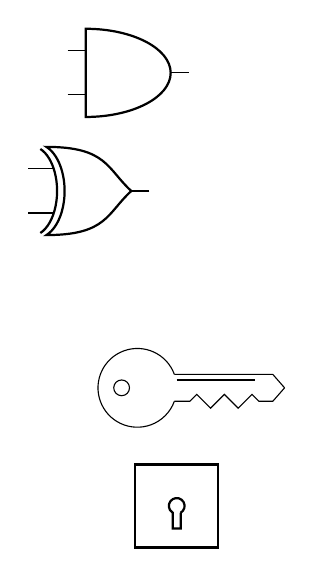
\begin{tikzpicture}
				\pause[0]
				\node[and port] (and) at (.5, 1.5){};
				\node[xor port] (xor) at (0, 0){};
				\draw (0,2) (0,-4.6);
				\only<2->{
					\bigkey{0,-2.5};
					\lockshape{.5,-4}{}
				}
			\end{tikzpicture}
		\end{column}
	\end{columns}
\end{frame}
\note{
To start describing how this works, I'm going to first explain boolean circuits and symmetric-key encryption. A boolean circuit is a bunch of logic gates like AND and XOR connected together by wires. Each gate is represented by a table that maps all possible inputs to their outputs. For usage in MPC, circuits can't have loops, so any looping algorithm will need its loops unrolled to be represented as a circuit. Circuits with these restraints can compute any math expression. (advance) After I go a bit deeper on boolean circuits, I'll talk about symmetric encryption. In particular, most implementations use AES, the Advanced Encryption Standard, which is the US government's chosen encryption scheme that has been well studied and has good hardware support. The specifics of the AES algorithm don't matter here, so it's fine to think about a cryptographic key as a literal key and a ciphertext as a locked box.

(advance) There's another basic concept that MPC builds with called an Oblivious Transfer, but I'll cover that when we get there.

}


\begin{frame}{Boolean Circuit}
	\centering
	\examplecircuit{1}{2}{3}{4}{5}
	\pause
	\begin{columns}
		\begin{column}{.3\textwidth}
			\centering
			\begin{tabular}{c c | c}
				A & B & C \\
				\midrule
				0 & 0 & 0 \\
				0 & 1 & 1 \\
				1 & 0 & 1 \\
				1 & 1 & 0 \\
			\end{tabular}
		\end{column}
		\pause
		\begin{column}{.3\textwidth}
			\centering
			\begin{tabular}{c c | c}
				A & B & C \\
				\midrule
				0 & 0 & 0 \\
				0 & 1 & 0 \\
				1 & 0 & 0 \\
				1 & 1 & 1 \\
			\end{tabular}
		\end{column}
		\pause
		\begin{column}{.3\textwidth}
			\centering
			\begin{tabular}{c c | c}
				A & B & C \\
				\midrule
				0 & 0 & 0 \\
				0 & 1 & 0 \\
				1 & 0 & 0 \\
				1 & 1 & 1 \\
			\end{tabular}
		\end{column}
	\end{columns}

\end{frame}
\note{
Let's start with a closer look at a circuit, and then I'll describe how MPC uses circuits while providing its security guarantees.

Here's an example of a simple boolean circuit. The input wires are on the left side labeled 1 and 2, the output wires are on the right, 4 and 5, and 3 is an internal wire. All the logic flows from left to right, with no outputs looping back to the left. Gates are referred to by their output number.

(advance) On the left is an XOR gate, number 3, and this table describes how it works. The two input wires on the left of the gate are the A and B columns, and the output is C. Each row of the table shows the output for one combination of inputs. This table, with the column headers replaced with wire labels, is all you need to describe this gate.

(advance) And here's a table for gate number 4, and AND gate, (advance) and here's the same table for gate number 5, which is also an AND gate.

This circuit is too small to be very useful. As a point of comparison, computing one block of a SHA-256 hash takes over 130,000 gates.

}


\begin{frame}{Symmetric-Key Encryption}
	\begin{columns}
		\begin{column}{.4\textwidth}
			\centering
			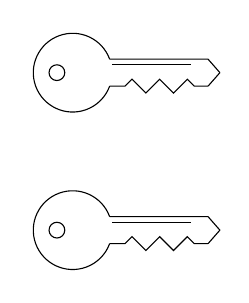
\begin{tikzpicture}
				\bigkey{0,1}
				\bigkey{0,-1}
			\end{tikzpicture}
		\end{column}
		\begin{column}{.6\textwidth}
			\begin{itemize}
				\item Each lock has one key
				\item Each box has two locks
				\item Put anything inside box
			\end{itemize}
		\end{column}
	\end{columns}
\end{frame}
\note{
We're going to talk about encryption here in a particular way. Everything will be encrypted with two keys, so you can picture a box that has two locks on it, and you need both keys to open it. You can put whatever you want inside the box, which is actually how things get interesting.

}


\begin{frame}
	\centering
	\Huge{Garbled Circuits}

	\pause
	\normalsize{Andrew Yao, 1986}
\end{frame}
\note{
Alright, now lets get on to the main event. I'm going to explain the most common technique for general-purpose multi-party computation, called Garbled Circuits.

(advance) This protocol was first described by Andrew Yao in 1986 at that year's IEEE Annual Symposium on Foundations in Computer Science. Since then, the cryptography community has worked out several major improvements to this protocol, including work by our own Dr. Rosulek in 2015. These improvements would make up another entire presentation, so I'll basically gloss over them for now.

}


\begin{frame}{What's Garbling?}
	\centering
	\newcommand*\changingline{}
	\newcommand*\changingbox{draw}
	\only<2->{\renewcommand{\changingline}{[dashed, black!10!white]}}
	\only<2->{\renewcommand{\changingbox}{black!10!white}}
	\begin{tikzpicture}[
		clearbox/.style={rectangle, draw, thick, minimum size=10mm},
		clearIO/.style={rectangle, thick, minimum size=10mm},
		garbledbox/.style={rectangle, draw, thick, minimum size=15mm,align=center},
		garbledIO/.style={rectangle, thick, minimum size=15mm, align=center},
		->,  % makes the edges directed
		>=stealth, % makes the arrow heads bold
		line width=.5mm,
		node distance=2cm,
		]
		\node[clearIO] (i)  {Input};
		\node[clearbox, right=of i,\changingbox] (c) {Circuit};
		\node[clearIO, right=of c] (o) {Output};
		\draw \changingline{} (i) -- (c);
		\draw \changingline{} (c) -- (o);
		\pause
		
		\node[garbledbox, below=of c] (gc) {Garbled \\ Circuit};
		
		\node at ($(c)+(0,-1.33cm)$) [
			top color=black!5!white,
			bottom color=red,
			single arrow,
			minimum height=2cm,
			minimum width=10mm,
			inner sep=0mm,
			single arrow head extend=.1mm,
			rotate=270, single arrow
		] {};

		\pause
		\node[garbledIO, below=of i] (gi) {Garbled \\ Input};
		\draw[red] (i)  -- (gi);
		\pause
		\draw[blue] (gi) -- (gc);
		\pause
		\node[garbledIO, below=of o] (go) {Garbled \\ Output};
		\draw[blue] (gc) -- (go);
		\pause
		\draw[red] (go) -- (o);

	\end{tikzpicture}
\end{frame}
\note{
Evaluating a circuit with the Garbled Circuits protocol requires starting with a normal circuit. Here's what that looks like. An input value is converted to true and false values on the left wires, these values are propagated through the circuit, and the output comes out the right side.

The garbled circuits protocol is split into two roles. There's the garbler, who I'll call Alice, and the evaluator, who I'll call Bob. Alice, who I'll show with red, has to first garble the circuit. (advance) I'll describe this process in a bit. Next, (advance) she works with Bob to transform the circuit's input into a garbled input. Bob, shown in blue, then puts this input into the garbled circuit (advance), and follows the calculation blindly to yield the (advance) garbled output. Finally, (advance), Alice helps him translate the garbled output back into the real output.

Even though there are two pretty different roles, shown here with colors, neither Alice nor Bob get any information about the other party's non-garbled input, so it's still secure.

}


\newcommand{\enc}[3]{\(\textrm{enc}(#1, #2, #3)\)}
\begin{frame}{Garbling a Gate}
	\centering
	\newcommand*\rhl{} % row highlight
	\only<2->{\renewcommand{\rhl}{\rowcolor{yellow}}}
	\begin{tabular}{c c | c}
		A & B & C \\
		\midrule
		\(A_0\) & \(B_0\) & \enc{A_0}{B_0}{0} \\
		\(A_0\) & \(B_1\) & \enc{A_0}{B_1}{0} \\
		\rhl\(A_1\) & \(B_0\) & \enc{A_1}{B_0}{0} \\
		\(A_1\) & \(B_1\) & \enc{A_1}{B_1}{1}
	\end{tabular}
	\vspace{1cm}

	Notation: \(\textrm{enc}(\textrm{key}_A, \textrm{key}_B, m)=\textrm{ciphertext}\)
%	\begin{tabular}{c c | c}
%		A & B & C \\
%		\midrule
%		0 & 0 & \(A\oplus B\) \\
%		0 & 1 & \(A\oplus B\) \\
%		1 & 0 & \(A\oplus B\) \\
%		1 & 1 & \(A\oplus B\)
%	\end{tabular}
\end{frame}
\note{
So how does Alice actually garble the circuit? She does it gate-by-gate, and this is where the locks and boxes come in. Let's consider an AND gate. Instead of using True and False in the input columns on the left of the table, Alice makes up some random strings. I used \(A_0\) here to indicate the random string that means false for input \(A\), and \(A_1\) is the random string that means true.

Then, she puts these in the truth table in place of the normal Trues and Falses on the left side.

Next, for each row, Alice uses these inputs as keys to encrypt that row's output. So the output column on the right of the table is replaced with ciphertexts, that each contain the gate's output for each possible input.

You can picture this as Alice making two keys for each gate input, one for True and one for False, and then making four boxes (one for each row of the table). She locks the output of the gate in each box using that box's input keys. This is the first part of the garbling. The second part is that she randomly permutes the rows of the table so that Bob can't figure out what the keys or the output mean based on their positions in the table.

(advance) If Bob only has the \(A_1\) and \(B_0\) keys, then he can only unlock the highlighted box that Alice gave him. Inside, he will find the gate output, which is 0 in this case. He can do this without learning that his first key corresponds to true and his second key corresponds to false. Alice has to know which key is which since she prepares the boxes, but Bob never gets this info.

}

\newcommand{\mathhl}[1]{\colorbox{yellow}{$\displaystyle #1$}}
\begin{frame}{Garbling a Circuit}
	\centering
	\examplecircuit{A}{B}{C}{D}{E}
	\pause
	\begin{tabular}{c c | c}
		A & B & C \\
		\midrule
		\(A_0\) & \(B_0\) & \enc{A_0}{B_0}{\mathhl{C_0}} \\
		\(A_0\) & \(B_1\) & \enc{A_0}{B_1}{\mathhl{C_1}} \\
		\(A_1\) & \(B_0\) & \enc{A_1}{B_0}{\mathhl{C_1}} \\
		\(A_1\) & \(B_1\) & \enc{A_1}{B_1}{\mathhl{C_0}}
	\end{tabular}
\end{frame}
\note{
We're talking about garbled circuits, though, not just garbled gates. So let's look at how garbled gates connect to each other. Here's the same circuit from before but with different wire labels.

Let's consider garbling that gate on the left, but instead of putting the true or false output of the gate into each box, (advance), we lock up the true or the false key that goes with the C wire! I highlighted the thing inside the locked boxes. Note that if you only look at the subscripts, this is the same as a normal truth table!

Remember that Alice made these keys and boxes and so she isn't allowed to evaluate the circuit. Bob can't see the subscripts, so all he knows is that he has \textit{a} key for wire C, and he doesn't know if it's the true or the false key. For the final wires D and E, though, Alice can just put the actual trues and falses in the boxes instead of making up a key. This is how Bob learns the answer to the calculation at the very end.

This means that if Alice makes all ten keys (two for each wire) and all twelve boxes (four for each gate), and then gives Bob just a single key for A and a single key for B, then Bob will be able to calculate the output of the circuit without knowing any of the values!

Perhaps you've noticed a problem, though. How can Bob get the keys for the A and B wires to start with? Let's say that Alice's input is wire A and Bob's input is wire B.

Alice generates the true and false keys for A and for B. She can just give Bob the right key for her own input A, since Bob doesn't know what it means. But she can't give Bob both keys for B or he would be able to speculatively execute the circuit and he might be able to figure out her input that way. Bob also can't just ask for the key that corresponds to his input, because then Alice would know his input!

}

\usetikzlibrary{arrows}
\begin{frame}{The Oblivious Transfer}
	\centering
	%\includegraphics[width=.8\textwidth]{ot.eps}
	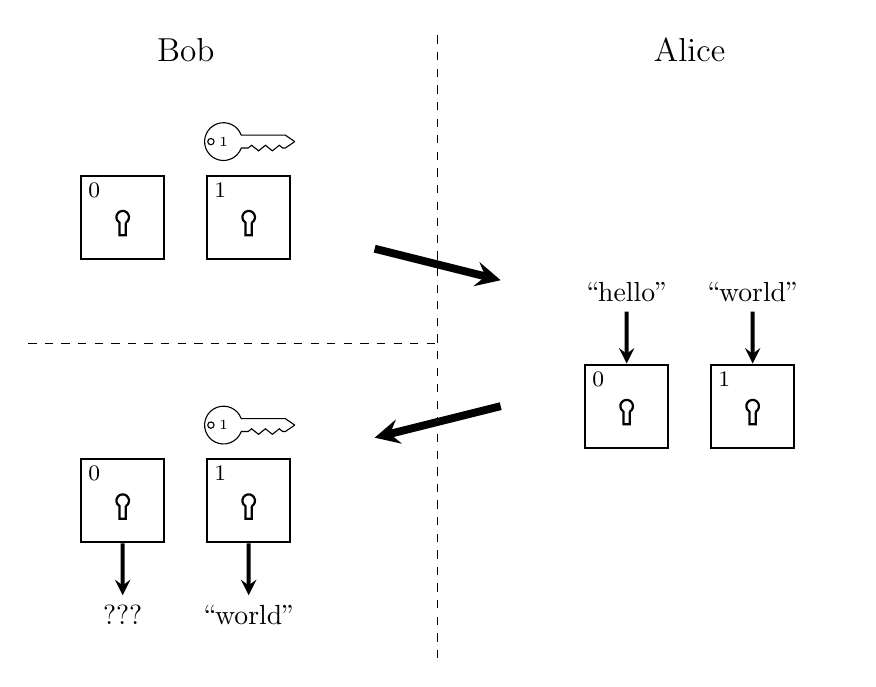
\begin{tikzpicture}[ scale=.8,
			IOarrow/.style={->, >=stealth, line width=.5mm},
			flowarrow/.style={->, >=stealth, line width=1mm, auto}
		]
		\draw[dashed] (0,-5) -- (0,5);

		\draw (-4,5) node [below] {\large{Bob}};
		\draw (4,5)  node [below] {\large{Alice}};
		\pause
		
		\lockshape{-5,2}{0} % step 1
		\lockshape{-3,2}{1}
		\pause
		% 1 -> 2 arrow
		\draw[flowarrow, bend right=20] (-1,1.5) -- (1,1);

		\lockshape{5,-1}{1} % step 2
		\draw (5,.5) node [above] (txt) {``world''};
		\draw[IOarrow] (txt) -- (lastBox);
		\lockshape{3,-1}{0}
		\draw (3,.5) node [above] (txt) {``hello''};
		\draw[IOarrow] (txt) -- (lastBox);
		\pause
		% key from step 1
		\littlekey{-3,3.2}{1}

		% horizontal divider
		\draw[dashed] (-6.5,0) -- (0,0) (6.5,0);
		% 2 -> 3 arrow
		\draw[flowarrow, bend right=20] (1,-1) -- (-1,-1.5);

		\lockshape{-5,-2.5}{0} % step 3
		\draw (-5,-4) node [below] (txt) {???};
		\draw[IOarrow] (lastBox) -- (txt);
		\lockshape{-3,-2.5}{1}
		\draw (-3,-4) node [below] (txt) {``world''};
		\draw[IOarrow] (lastBox) -- (txt);
		\littlekey{-3,-1.3}{1}

	\end{tikzpicture}
\end{frame}
\note{
The solution is a really fun cryptographic primitive called an Oblivious Transfer, or OT. If Alice and Bob perform an OT, then Bob can ask for just one key, and Alice sends it to him. The cool part is that Alice doesn't know which one he asked for, and Bob doesn't know anything about the key he didn't receive!

(advance) You can picture this as Bob sending Alice two empty boxes, labeled 0 and 1. (advance) Alice puts messages in each box, locks them, and sends them back. (advance) But Bob only made the key to box 1, a choice he made before sending anything to Alice. Alice doesn't know which message Bob got, since the locks on the boxes look the same to her. Bob doesn't learn anything about the other message since this whole thing is set up so that he can only ever open one box.

Now imagine that the messages that Alice puts in the boxes are actually the True and False keys for an input wire to the circuit. This is how Bob can ask for the keys he needs without Alice learning his input.

}

\begin{frame}{Putting it All Together}
	\pause
	\begin{itemize}[<+->]
		\item Alice generates keys and boxes
		\item Alice sends her keys to Bob
		\item Bob gets his keys with OT
		\item Bob evaluates the circuit
	\end{itemize}
\end{frame}
\note{
So let's put all those pieces together. First, (advance) Alice garbles every gate by generating a bunch of keys and boxes, with each box containing a key to a later box. Next, (advance) Alice sends the keys that correspond to her inputs over to Bob, since he doesn't know which keys mean True and which mean False. Then, (advance) Bob uses an oblivious transfer to get the True and False keys for his input from Alice. Since it's oblivious, Alice doesn't know which keys he got, so neither of them know the other's inputs.

Finally, (advance) Bob evaluates the circuit by repeatedly opening boxes to get more keys. There are ways to make sure he shares the answer with Alice at the end, but that's out of scope right now.

}

\begin{frame}{Review}
	\centering
	\newcommand*\changingline{}
	\newcommand*\changingbox{draw}
	\only<2->{\renewcommand{\changingline}{[dashed, black!10!white]}}
	\only<2->{\renewcommand{\changingbox}{black!10!white}}
	\begin{tikzpicture}[
		clearbox/.style={rectangle, draw, thick, minimum size=10mm},
		clearIO/.style={rectangle, thick, minimum size=10mm},
		garbledbox/.style={rectangle, draw, thick, minimum size=15mm,align=center},
		garbledIO/.style={rectangle, thick, minimum size=15mm, align=center},
		->,  % makes the edges directed
		>=stealth, % makes the arrow heads bold
		line width=.5mm,
		node distance=2cm,
		]
		\node[clearIO] (i)  {Input};
		\node[clearbox, right=of i,\changingbox] (c) {Circuit};
		\node[clearIO, right=of c] (o) {Output};
		\draw \changingline{} (i) -- (c);
		\draw \changingline{} (c) -- (o);
		\pause
		
		\node[garbledbox, below=of c] (gc) {Garbled \\ Circuit};
		
		\node at ($(c)+(0,-1.33cm)$) [
			top color=black!5!white,
			bottom color=red,
			single arrow,
			minimum height=2cm,
			minimum width=10mm,
			inner sep=0mm,
			single arrow head extend=.1mm,
			rotate=270, single arrow
		] {};

		\pause
		\node[garbledIO, below=of i] (gi) {Garbled \\ Input};
		\draw[red] (i)  -- (gi);
		\pause
		\draw[blue] (gi) -- (gc);
		\pause
		\node[garbledIO, below=of o] (go) {Garbled \\ Output};
		\draw[blue] (gc) -- (go);
		\pause
		\draw[red] (go) -- (o);

	\end{tikzpicture}
\end{frame}
\note{
Alright, let's review. Here's what it looks like to evaluate a normal boolean circuit. Or any computation, really. We're just representing it as a boolean circuit since that's how garbled gates work.

(advance) Alice is the garbler, and her job at the beginning is to transform this circuit in a special way that we call garbling. The circuit still encodes all the same logic, but once it's garbled, you need a lot of insider information to know any intermediate values on wires inside the circuit.

(advance) Since the circuit is in this special transformed representation, and Alice is the only one who knows what the transformation was, she needs to play a role in turning normal inputs into garbled inputs. Values on wires are usually just True or False, but after the transformation, they're all just random strings. Alice keeps track of the transformation, so she knows which random strings mean what. Since she has all the secrets, she can't be the one to evaluate the circuit, since then she would learn Bob's inputs.

Instead, Bob needs to be the one that does the evaluations. The problem is that Bob doesn't know what garbled inputs to feed the garbled circuit. Alice can directly send the keys that correspond to her input to Bob, and Bob doesn't learn anything about Alice's inputs since they're random anyway. Bob, on the other hand, needs a more clever way to get his keys. This is the part with the oblivious transfer. Bob can ask for the keys he needs one-by-one for each bit of his input, and since the transfer is oblivious, Alice doesn't know if he's receiving the keys that correspond to True or to False. Also, Bob only receives one key for each of his input wires, so he doesn't learn anything about other possible circuit outputs given Alice's inputs.

(advance) Once Bob has all the keys, he can start unlocking boxes. Alice sent him a collection of boxes that together are a garbled circuit. Each box has two key holes, one for each input wire to a gate. Bob can just unlock any boxes he has keys for, and inside most of the boxes will be more keys, representing the output of that gate. When he does this, Bob is executing the circuit blindly without learning anything about the values until the very end,

(advance) where the boxes instead have the plaintext True or False values inside. The garbled circuit is like a black box that Bob drops his keys into, and then he just turns the crank until the answer comes out the other side.

(advance) Alice made all the boxes, so she's the one that has to put the circuit outputs in the last boxes on the right side of the circuit. It's her knowledge of the garbling transformation that's required to convert the answer from garbled nonsense to the result of the calculation.

The vertical arrows in this diagram are transformations to and from the garbled execution space. The horizontal arrows are computations within the garbled execution space. Since Alice knows about the transformation, she can't be the one to do the execution. Since Bob has all the inputs, he can't learn anything about the transformation. Together, though, they can perform the computation without either of them learning anything about the computation, including each other's inputs, except the final result.

}


\maketitle
\note{
So there you have it. A basic explanation of Garbled Circuits, one of the weirder topics on cryptography. There's a lot more to learn, like ways to reduce the number of boxes that Alice needs to send Bob per gate, and ways to deal with more than two people who want to perform a computation together. But all of that would take much longer than twenty minutes to explain!

Thank you for listening. My name is Gabriel and this was an introduction to Multi-Party Computation.

}


\end{document}
